\begin{appendix}
\chapter{Anexo: Detalles del código}\label{Anexo_codigo}

  \par Se decidió realizar todo el desarrollo en el lenguaje de programación
    \textit{Python} por su simplicidad, buen desempeño y su extensa
    comunidad activa. Esto facilita el desarrollo e incrementa la velocidad
    de producción. El proyecto está disponible
    en \url{https://github.com/juansca/modeling-mosquitos} y en su sección
    inicial se pueden encontrar instrucciones para su instalación.
    A continuación se describirán
    algunos aspectos que se consideran relevantes de los distintos módulos,
    sin entrar en detalles.

  \par El módulo \verb|data| por un lado tiene un archivo llamado
    \verb|constants.py| en donde se definen algunas constantes que
    son dependientes del conjunto de datos que se utilizará. Es importante
    dado que es allí en donde se especifican los \textit{features} (o
    columnas) que se utilizarán como input para predicción.
    A su vez, en dicho módulo, el archivo \verb|data_cleaner.py|
    posee una clase llamada \verb|DataCleaner| que es la encargada de
    realizar la limpieza de los datos. Para realizar la limpieza de los
    datos se debe ejecutar el script \verb|scripts/clean_data.py|, el
    cual arroja el siguiente instructivo:

    \begin{lstlisting}
    $ python data/scripts/clean_data.py --help

    Clean Data.

    Usage:
      ./clean_data.py -i <file> -o <dir> [--p_eval <float>] [--instances <n>] [--overlap <f>]

    Options:
      -i <file>              Evaluate dataset path
      -o <dir>               Directory where the evaluation plot result will be
                             saved
      --p_eval <float>       Percentage to evaluation dataset. [default: 0.2]
      --instances <n>        Number of instances to generate from data
                             [default: 1]
      --overlap <f>          Percentage of overlapping between the instances.
                             [default: 0]

    \end{lstlisting}


  \par Por otro lado, el módulo \verb|models| tiene un archivo llamado
    \verb|models.py| en el cual se declaran los modelos
    que se utilizarán para el modelado. Es importante que estos modelos
    sigan la estructura ahí utilizada para que los demás módulos los
    puedan utilizar correctamente.

  \par Además, allí se encuentra el \textit{script} de entrenamiento,
    \verb|scripts/train.py|, que entrena el modelo elegido con el conjunto
    de datos dado e imprime por linea de comandos un conjunto de
    estadísticas que resultan de realizar validación cruzada sobre
    los datos brindados por el usuario para dicha tarea. Ésto resulta útil
    para tener una noción del desempeño del modelo.
    Éste script devuelve la siguiente documentación de uso:
    \begin{lstlisting}
    $ python models/scripts/train.py --help

    Train a model

    Usage:
      ./train.py -i <file> --model <model> [-p <file>]
      ./train.py -h | --help

    Options:
      -i <file>         Train/Val dataset path
      --model <model>   Model you want to train, is mandatory that it was on
                        models.py file.
      -p <file>         CSV file where are saved the hyperparameters
                        (in case of tunning module was used).
    \end{lstlisting}

  \par Por otra parte, el módulo posee un \textit{script} de evaluación,
  que, además de imprimir por linea de comandos el valor del Error Cuadrático Medio de la
  evaluación, genera un gráfico con la curva real y la curva predicha
  por el modelo y lo guarda en un directorio. A su vez, guarda un
  archivo \verb|csv| con los valores reales y los generados por el modelo
  facilitando así, la posterior manipulación del mismo.
  La documentación de ayuda para su utilización es:
  \begin{lstlisting}
  $ python models/scripts/eval.py --help

  Evaluate a model

  Usage:
    ./eval.py -i <file> -m <model> [-o <file>]

  Options:
    -i <file>         Evaluate dataset path
    -m <model>        Model you want to evaluate as pickle format
    -o <dir>          Directory where the evaluation plot result will be saved

  \end{lstlisting}

\par Finalmente, el sistema desarrollado posee el módulo \verb|tunning|.
  Allí se realiza el ajuste de hiperparámetros de los modelos.
  Existe varios archivos en ese módulo que son los que hacen de interfaz
  con la herramienta \textit{irace}. Algo que cabe destacar aquí es el
  directorio \verb|parameters|. Allí se colocan los posibles
  (o intervalos de) valores que generan el espacio de hiperparámetros
  donde la herramienta buscará los óptimos para cada modelo. Además,
  \textit{irace}, usará las instancias de datos en \verb|instances|
  para realizar dicha tarea. Algo de suma importancia es que
  los datos utilizados para generar los últimos conjutos deben ser distintos
  a los que se usarán posteriormente en el entrenamiento o validación de
  los modelos. Esto se debe a que si no, se puede generar una dependencia
  de los datos y podría llevar al sobre-ajuste (\textit{overfitting})\footnote{Una
  analogía clara es que el modelo aprende "de memoria" los datos en vez de
  comprenderlos. Esto lleva a una muy pobre capacidad de generalización.}.
  El \textit{script} que se debe ejecutar para hacerlo es \verb|tune_params.py|.
  Su documentación de uso es:
  \begin{lstlisting}
  $ python tunning/tune_params.py --help

  Tune parameters for given models.

  Usage:
    tune_params.py --model <name>

  Options:
    --model <name>           model name to tune params.
                             Options: svr, rdmforest, pcardmforest, dtr, knnr,
                             mlpr, svr, pcaknnr, pcadtr.
                             If you want to tune all the models together, just
                             put on this parameter 'all'.
    --help                   show this screen

  \end{lstlisting}
\par Por último, en la Figura \ref{fig:proyecto_modelado} se puede observar
  la estructura general del proyecto.

  \begin{figure}[hbt]
  \centering%
  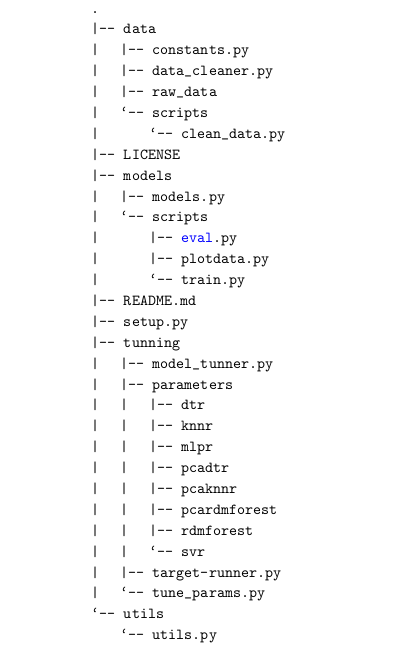
\includegraphics[width=0.6\textwidth]{images/proyecto_modeling}%
  \caption{Sistema para el ajuste de parámetros y modelado}\label{fig:proyecto_modelado}
  \end{figure}

\end{appendix}
